\chapter{全球变化与生物圈}\label{ch:b2:global-change}

1851 年至 1858 年间，亨利·梭罗走遍了
马萨诸塞州康科德周围的树林与草地，逐一记下约
五百种植物中每一种首次开花的日期。一个半世纪后，
植物学家带着他的笔记，回到同一批地点。
梭罗记录的高丛蓝莓于 5月11日开放，如今在
4月12日即开放；整个植物区系平均
比他那个年代提前了十天，与春季升温 \qty{2.4}{\celsius}
相呼应；他记录的物种中有四分之一已从康科德消失——
不是随机的，而是那些开花时间无法跟上
气温变化的物种。前几章给出了其中的机制：
\cref{ch:b2:biogeochemical-cycles}中的循环，
\cref{ch:b2:population-genetics}中的选择与漂变，
\cref{ch:b2:speciation}中的竞争与物种形成，以及\cref{ch:b2:living-soil}中的\omterm{def:b2:living-soil:soil}{土壤}。
本章用数字量化一个物种改变大气与海洋化学组成时，
生物所经历的变化：每吨碳导致多少升温，每升温
一度春季提前多少天，上坡迁移多少米，
海水中有多少酸，每公顷有多少物种消失——
以及这些数字对
下一个世纪意味着什么。

\section{物理变化}

\begin{proposition}[升温与累积排放成正比]\label{prop:b2:global-change:tcre}
\index{全球变暖}\index{累积排放}\index{碳预算}\index{温室效应}
二氧化碳吸收地面放出的红外线，并将其中的一部分
反射回地面；\ensuremath{\mathrm{CO_2}} 越多，地表越暖，约
\qty{3}{\celsius}，浓度每翻一番（待海洋充分吸热之后）
（\emph{气候敏感度}）。由于温度对
\ensuremath{\mathrm{CO_2}} 的响应与浓度呈对数关系，而排放中
留存于大气的份额随浓度升高而下降，两者的曲率
近乎相互抵消，因此全球平均升温在很好的近似下，
\emph{与\omterm{prop:b2:global-change:tcre}{累积排放}的碳量呈线性关系}，
而与排放时间无关：
\[
\Delta T \approx \lambda\,C_{\text{累积}}, \qquad \lambda \approx
\qty{1.65}{\celsius} \text{ 每 } \qty{1000}{GtC}
\]
（\qty{0.45}{\celsius} 对应每 \qty{1000}{Gt} \ensuremath{\mathrm{CO_2}}）。
自 1850 年以来排放的约 \qty{700}{GtC} 已使地球
升温 \qty{1.2}{\celsius}，由此关系可为每个升温目标给出一个预算：
\qty{1.5}{\celsius} 的目标合计约允许 \qty{900}{GtC}，
比已排放量多 \qty{200}{GtC}，约相当于
以当前速率排放二十年。升温并不均匀：陆地上为全球平均的两倍，
北极则为三倍；夜间升温多于白天；它还伴随着
其他变化：降雨更强、干旱更长，海平面
每年上升 \qty{4}{mm}，夏季冰量小了五分之一，
而海洋已吸收了 \qty{90}{\%} 的热量，
以及四分之一的碳。
\end{proposition}
\begin{proof}[证据]
这一比例关系在各种复杂程度的气候模式中
均有发现，并为观测记录所证实：将 1850 年以来的升温对
与\omterm{prop:b2:global-change:tcre}{累积排放}量作图，得到一条
穿越各个十年的直线。\omterm{prop:b2:global-change:tcre}{温室效应}本身可从轨道上测量：
卫星观测到地球放出的红外线，并
扣除其中 \ensuremath{\mathrm{CO_2}}、甲烷与水蒸气的吸收带，
这一扣除在 1970 年至 2020 年间加深，加深幅度恰好
与这些气体增加所预测的一致。同位素与
\cref{ch:b2:biogeochemical-cycles}中的氧含量下降，共同将额外的
\ensuremath{\mathrm{CO_2}} 与化石燃料联系起来。
\end{proof}

\begin{omfigure}
\begin{tikzpicture}
\begin{axis}[
  width=0.88\linewidth, height=5.6cm,
  axis x line=bottom, axis y line=left,
  xmin=1845, xmax=2030, ymin=-0.3, ymax=1.5,
  xlabel={十年}, ylabel={自 1850--1900 年以来的升温（\unit{\celsius}）},
  xlabel style={font=\small, at={(axis description cs:0.5,-0.13)}, anchor=north},
  ylabel style={font=\small},
  tick label style={font=\small}, xtick={1850,1900,1950,2000}, ytick={0,0.5,1,1.5},
  scaled x ticks=false, x tick label style={/pgf/number format/1000 sep=},
  clip=false,
]
\addplot[ybar, bar width=7pt, fill=omThm!50, draw=omThm] coordinates {
(1855,0.00) (1865,-0.04) (1875,0.02) (1885,-0.06) (1895,-0.02) (1905,-0.10) (1915,-0.06) (1925,0.05) (1935,0.15) (1945,0.25) (1955,0.15) (1965,0.15) (1975,0.18) (1985,0.40) (1995,0.55) (2005,0.78) (2015,1.02) (2023,1.28)};
\node[font=\scriptsize, anchor=west, align=left] at (axis cs:1850,1.2) {每根柱为该十年的平均值；最后一根为 2020--2024 年 \\ 排放 \qty{700}{GtC}，$\qty{1.65}{\celsius}/\qty{1000}{GtC}$：\qty{1.2}{\celsius}};
\end{axis}
\end{tikzpicture}

{\small 按十年统计的全球平均地表气温，相对于
十九世纪后半叶的水平。最近四个十年每个
都创下纪录，1970 年以来的升温速率为每
十年 \qty{0.2}{\celsius}。}
\end{omfigure}

\section{物候日历}

\begin{theorem}[积温与春季提前]\label{thm:b2:global-change:phenology}
\index{物候学}\index{积温}\index{热时间}\index{物候错配}
许多植物与外温动物生命中的事件——芽萌发、
开花、卵孵化、羽化——都发生在累积的
\emph{\omterm{thm:b2:global-change:phenology}{热时间}}，即自起始日期以来每日高于基温 $T_b$ 的温度之和
（\emph{\omterm{thm:b2:global-change:phenology}{积温}}）达到
固定总量 $K$。若春季气温线性上升，$T(t) = T_b
+ b\,(t - t_0)$，以每日 $b$ 度的速率升温，自越过
基温的那天 $t_0$ 起，事件发生于
\[
t^{*} = t_0 + \sqrt{2K/b},
\]
若均匀升温 $\Delta T$，则越过基温的日期提前
$\Delta T/b$ 天，事件随之提前。取 $b \approx
\qty{0.1}{\celsius}$ 每天，\emph{每升温一度
约提前十天}。各物种的 $T_b$、$K$ 不同，并且是否还利用
日长（升温并不改变日长）——于是一个食物链中的
各成员以不同速率提前，它们的
时间逐渐错开，形成\emph{\omterm{thm:b2:global-change:phenology}{物候错配}}：毛毛虫与
必须以之喂养雏鸟的鸟类。
\end{theorem}
\begin{proof}
自 $t_0$ 起的\omterm{thm:b2:global-change:phenology}{积温}：$\int_{t_0}^{t}(T - T_b)\,\mathrm{d}t' =
b\,(t - t_0)^{2}/2$，等于 $K$ 的条件是 $t - t_0 = \sqrt{2K/b}$。
升温 $\Delta T$ 即将 $T$ 替换为 $T + \Delta T$：
基温被越过的时间提前 $\Delta T/b$ 天，累积过程
自那天起完全相同，也同样提前 $\Delta T/b$ 天完成。（若
升温同时使 $b$ 增大，则区间 $\sqrt{2K/b}$
也随之缩短。）以日长为信号的物种日期不变，
以\omterm{thm:b2:global-change:phenology}{积温}为信号的物种则移动，两者之间的间隔增加 $\Delta T/b$。
\end{proof}
\begin{proof}[证据]
梭罗记录的康科德植物区系，以及马舍姆家族的
1736 年至 1947 年间在诺福克所记的二十七种春季物候迹象，
两者都显示开花与展叶提前 \qtyrange{3}{6}{d}
每春季升温一度。京都樱花的花期由宫廷日记记录，
自九世纪起，大致稳定在四月中旬，持续了一千年，
1900 年以来已提前到四月上旬，
有记录以来最早的日期出现在 2020 年代。在荷兰，
栎树毛毛虫的数量高峰如今比 1985 年提前了两周；
大山雀受同样暖意的引导，已跟上节奏，但捕蝇鸟
依日长安排自非洲迁徙的时间，
仍如往常抵达，却发现高峰已过——其种群
数量在错配最严重之处下降了 \qty{90}{\%}（博特等人，
2006）。
\end{proof}

\begin{omfigure}
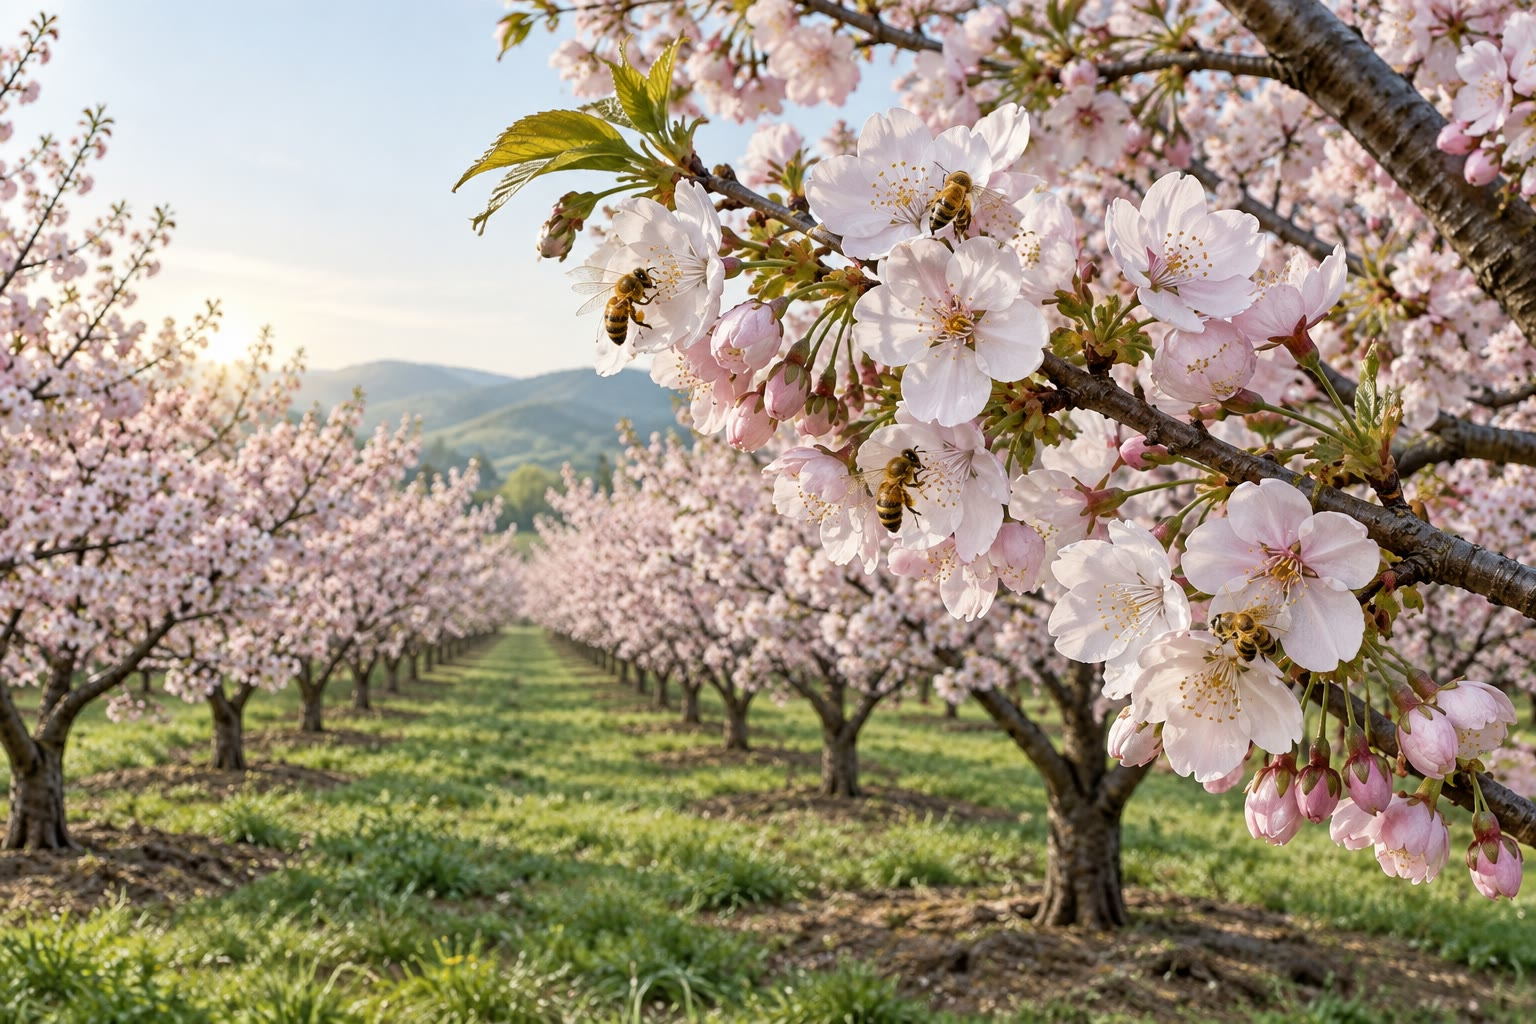
\includegraphics[width=0.62\linewidth]{images/book4/ai/b4-27-phenology-cherry.jpg}

{\small 盛开的樱桃园。京都樱花的花期在日记中记载了十二个世纪，
如今开花时间早于 1900 年前的任何一年——
而为它们\omterm{def:b2:angiosperm-reproduction:pollination}{传粉}的蜜蜂，
也必须在同一天飞行。}
\end{omfigure}

\begin{omfigure}
\begin{tikzpicture}
\begin{axis}[
  width=0.74\linewidth, height=5.4cm,
  axis x line=bottom, axis y line=left,
  xmin=0, xmax=100, ymin=0, ymax=14,
  xlabel={自 3 月 1 日起的天数}, ylabel={日平均气温（\unit{\celsius}）},
  xlabel style={font=\small, at={(axis description cs:0.5,-0.13)}, anchor=north},
  ylabel style={font=\small},
  tick label style={font=\small}, xtick={0,20,40,60,80,100},
  legend style={font=\scriptsize, at={(0.03,0.97)}, anchor=north west, draw=none},
  clip=false,
]
\addplot[very thick, omDef, domain=0:100, samples=2] {2 + 0.1*x};
\addlegendentry{升温前的春季}
\addplot[very thick, omThm, domain=0:100, samples=2] {3 + 0.1*x};
\addlegendentry{春季升温 \qty{1}{\celsius}}
\draw[dashed, gray] (axis cs:0,5) -- (axis cs:100,5); \node[font=\scriptsize, anchor=south east] at (axis cs:100,5) {基准温度 $T_b = \qty{5}{\celsius}$};
\fill[omDef, opacity=0.15] (axis cs:30,5) -- (axis cs:93,5) -- (axis cs:93,11.3) -- cycle;
\fill[omThm, opacity=0.15] (axis cs:20,5) -- (axis cs:83,5) -- (axis cs:83,11.3) -- cycle;
\draw[<->, thick] (axis cs:83,1.6) -- (axis cs:93,1.6); \node[font=\scriptsize, anchor=south] at (axis cs:88,1.8) {10 天};
\draw[dotted] (axis cs:93,0) -- (axis cs:93,5); \draw[dotted] (axis cs:83,0) -- (axis cs:83,5);
\node[font=\scriptsize, anchor=south, align=center] at (axis cs:62,11.4) {$K = 200$ 度日 \\ （阴影面积）};
\end{axis}
\end{tikzpicture}

{\small 度日。当温度线与基准线之间的阴影面积
达到 $K$ 时事件发生；春季每升温 1 摄氏度，
越过基准线的时间便提前 10 天，\omterm{thm:b2:global-change:phenology}{积温}
的累积也提前 10 天。}
\end{omfigure}

\section{地图：分布区移动}

\begin{proposition}[等温线移动，物种随之而移]\label{prop:b2:global-change:range}
\index{分布区移动}\index{气候速度}\index{气温垂直递减率}
沿海拔每千米，气温下降约 \qty{6.5}{\celsius}，
温带地区沿纬度每百千米下降约 \qty{0.65}{\celsius}；
因此，升温 \qty{1}{\celsius} 使每条等温线
向高处上移约 \qty{150}{m}，并向极地方向移动约
\qty{150}{km}。受温度限制的物种，其分布边界
若条件允许便随等温线移动：数百个所研究物种的平均值
每十年向上移动 \qty{11}{m}，向极地移动 \qty{17}{km}，
自 1970 年以来，即与等温线移动速度相当，而
最快的物种——流动性强、适应面广、寿命短——能够超越它们，
而树木的\omterm{def:b2:angiosperm-reproduction:seed}{种子}每年仅能传播数米，以及已
处于山顶或极地的物种则无法跟上：山顶无处可升，
每升温一摄氏度，每个分布区都失去最高的
\qty{150}{m}。海洋物种没有屏障阻隔，
热限制更为敏感，移动最快，每十年可达数十千米；
鳕鱼、鲭鱼及依赖它们的渔业已向北移动，
跨越整片海域。分布区的上缘向前推进，下缘
随升温而后退，同时新的竞争者从下方到来，
任一地点的群落，由彼此从未相遇的物种
重新组合而成。
\end{proposition}
\begin{proof}[证据]
帕尔马桑（1996）重新调查了埃迪斯豹蛱蝶
在其北美西部的分布区内：南缘和低海拔的种群已灭绝，
北缘和高海拔的种群则繁茂兴旺，整个分布区
已向北移动 \qty{92}{km}，向上移动 \qty{124}{m}
——首次被证实追踪等温线的物种。
勒努瓦等（2008）
比较了法国山区 1905--1985 年与 1986--2005 年的森林植物调查，
171 个物种的最适海拔已
每十年上升了 \qty{29}{m}。陈等（2011）在
涵盖两千个物种的研究中发现，移动速度
比此前估计快两至三倍，且与当地升温成正比。
\end{proof}

\begin{omfigure}
\begin{tikzpicture}[every node/.style={font=\scriptsize}, >=stealth]
  \fill[gray!25] (0,0) -- (3.5,4.2) -- (7,0) -- cycle;
  \draw[thick] (0,0) -- (3.5,4.2) -- (7,0);
  \foreach \y/\lab in {1.0/{\qty{12}{\celsius}}, 2.2/{\qty{8}{\celsius}}, 3.4/{\qty{4}{\celsius}}} { \draw[omDef, thick] ({\y/1.2},\y) -- ({7-\y/1.2},\y) node[right] {\lab}; }
  \foreach \y in {1.15,2.35,3.55} { \draw[omThm, thick, dashed] ({\y/1.2},\y) -- ({7-\y/1.2},\y); }
  \node[omThm, anchor=west, align=left] at (7.6,3.7) {虚线：同一等温线 \\ 升温 \qty{1}{\celsius} 后，\\ 上移 \qty{150}{m}};
  \fill[omProp!50] (0.83,1.0) -- (6.17,1.0) -- (5.17,2.2) -- (1.83,2.2) -- cycle;
  \node[align=center] at (3.5,1.6) {某物种的分布带，\\ \qtyrange{1000}{1200}{m}};
  \draw[->, thick, omExo!80!black] (1.1,2.2) -- (1.1,2.9); \node[omExo!80!black, anchor=east, align=right] at (0.95,2.55) {分布带上移 \\ 并缩小};
  \node[anchor=north] at (3.5,-0.1) {一座山：面积随海拔升高而缩小，山顶已无更高处};
\end{tikzpicture}

{\small 山地上的\omterm{prop:b2:global-change:range}{分布区移动}。每升温一摄氏度，等温线
上移 \qty{150}{m}；物种的分布带随之向上，进入
面积更小的区域，而已处于山顶的分布带则消失。}
\end{omfigure}

\section{海洋：酸化与高温}

\begin{theorem}[酸化]\label{thm:b2:global-change:acid}
\index{海洋酸化}\index{碳酸盐体系}\index{饱和度}\index{珊瑚白化}
二氧化碳溶于海水生成碳酸，碳酸
发生解离：$\ensuremath{\mathrm{CO_2}} + \ensuremath{\mathrm{H_2O}} \rightleftharpoons \ensuremath{\mathrm{H^{+}}} +
\ensuremath{\mathrm{HCO_3^{-}}}$，其中 $[\ensuremath{\mathrm{H^{+}}}][\ensuremath{\mathrm{HCO_3^{-}}}]/[\ensuremath{\mathrm{CO_2}}] = K_1$。
碳酸氢根是海洋中最大的碳库，
由碱度维持近乎恒定，因此
\[
[\ensuremath{\mathrm{H^{+}}}] \propto p_{\ensuremath{\mathrm{CO_2}}}, \qquad
\Delta\mathrm{pH} \approx -\log_{10}\frac{p_{\ensuremath{\mathrm{CO_2}}}}{p_0}
\]
——更精确地应为比值的 $-0.9\log_{10}$，因为碳酸氢根
略有上升。自 280 到 \qty{420}{ppm}，表层 pH 下降了
$0.15$，由 $8.2$ 降至 $8.05$：氢离子
增加了 \qty{40}{\%}；若达 \qty{800}{ppm}，则将下降 $0.4$。额外的
氢离子消耗碳酸根，$\ensuremath{\mathrm{H^{+}}} + \ensuremath{\mathrm{CO_3^{2-}}} \to \ensuremath{\mathrm{HCO_3^{-}}}$，而
碳酸钙的\emph{\omterm{thm:b2:global-change:acid}{饱和度}} $\Omega$——
即钙与碳酸根浓度的乘积，除以
溶度积——按比例下降：文石质的贝壳与骨骼
（珊瑚、翼足类）在 $\Omega > 3$ 时易于形成，
在接近 1 时较难形成，低于它则溶解；热带表层
工业化前为 $\Omega \approx 4$，如今为 3，
在 \qty{560}{ppm} 时降至 2，而寒冷、富含
\ensuremath{\mathrm{CO_2}} 的极地表层海水率先降至 1。
\end{theorem}
\begin{proof}
由平衡关系，$[\ensuremath{\mathrm{H^{+}}}] = K_1[\ensuremath{\mathrm{CO_2}}]/[\ensuremath{\mathrm{HCO_3^{-}}}]$，且
$[\ensuremath{\mathrm{CO_2}}]$ 正比于 $p_{\ensuremath{\mathrm{CO_2}}}$，依亨利定律；
$[\ensuremath{\mathrm{HCO_3^{-}}}]$ 不变时，$[\ensuremath{\mathrm{H^{+}}}]$ 正比于
$p_{\ensuremath{\mathrm{CO_2}}}$，而 $\mathrm{pH} = -\log_{10}[\ensuremath{\mathrm{H^{+}}}]$ 的变化量为
比值的 $-\log_{10}$。第二个平衡式为 $[\ensuremath{\mathrm{H^{+}}}][\ensuremath{\mathrm{CO_3^{2-}}}]/[\ensuremath{\mathrm{HCO_3^{-}}}]
= K_2$，给出 $[\ensuremath{\mathrm{CO_3^{2-}}}] \propto 1/[\ensuremath{\mathrm{H^{+}}}] \propto
1/p_{\ensuremath{\mathrm{CO_2}}}$，故 $\Omega$ 随 $p_{\ensuremath{\mathrm{CO_2}}}$ 升高而下降，且
$[\ensuremath{\mathrm{H^{+}}}]$ 升高 \qty{40}{\%}，相当于碳酸根下降
\qty{30}{\%}。（完整的化学关系，包括碳酸氢根的变化与
离子活度，给出因子 $0.9$ 及观测数值；
此部分由本科三年级分册讨论。）
\end{proof}
\begin{proof}[证据]
夏威夷以北的海洋观测站每月测量表层 pH，
自 1988 年以来，pH 每年下降 $0.0018$，
与其上方莫纳罗亚站的 \ensuremath{\mathrm{CO_2}} 同步变化，正如化学所要求的。
翼足类——即海中的“蜗牛”，是鲑鱼与鲸的食物——
在太平洋沿岸采集的样本显示，其文石质贝壳
出现凹坑并正在溶解，那里上升流将 $\Omega <
1$ 的海水带至表层。\omterm{thm:b2:global-change:acid}{珊瑚白化}是高温所致，而非酸化：当
海水高出夏季最高值 \qty{1}{\celsius} 并持续数
周，珊瑚便排出共生藻而饥饿；大堡礁
曾于 1998、2002、2016、2017、2020、2022 和 2024 年白化，
自 1995 年以来，其珊瑚覆盖率已减少一半。
\end{proof}

\begin{omfigure}
\begin{tikzpicture}
\begin{axis}[
  width=0.68\linewidth, height=5.4cm,
  axis x line=bottom, axis y line=left,
  xmin=250, xmax=1000, ymin=7.6, ymax=8.3,
  xlabel={大气 \ensuremath{\mathrm{CO_2}} (ppm)}, ylabel={表层 pH},
  xlabel style={font=\small, at={(axis description cs:0.5,-0.13)}, anchor=north},
  ylabel style={font=\small},
  tick label style={font=\small}, xtick={280,420,560,800,1000}, ytick={7.6,7.8,8.0,8.2},
  clip=false,
]
\addplot[very thick, omDef, domain=250:1000, samples=60] {8.2 - 0.9*log10(x/280)};
\fill[omDef] (axis cs:280,8.2) circle (2pt); \node[font=\scriptsize, anchor=south west] at (axis cs:285,8.2) {1750};
\fill[omThm] (axis cs:420,8.04) circle (2pt); \node[font=\scriptsize, anchor=south west] at (axis cs:425,8.04) {2020 年代：$-0.15$，$+\qty{40}{\%}$ \ensuremath{\mathrm{H^{+}}}};
\fill[omThm] (axis cs:800,7.79) circle (2pt); \node[font=\scriptsize, anchor=south west] at (axis cs:805,7.79) {高排放下的 2100 年};
\node[font=\scriptsize, anchor=north east, align=right] at (axis cs:1000,8.28) {$\Omega_{\text{文石}}$，热带：\\ 1750 年为 4，现在为 3，在 \qty{560}{ppm} 时为 2};
\end{axis}
\end{tikzpicture}

{\small 表层海水 pH 随大气二氧化碳的变化，
$\mathrm{pH} = 8.2 - 0.9\log_{10}(p/280)$。此标度为
对数标度：pH 每下降 0.1 个单位，氢离子
便多出四分之一。}
\end{omfigure}

\begin{omfigure}
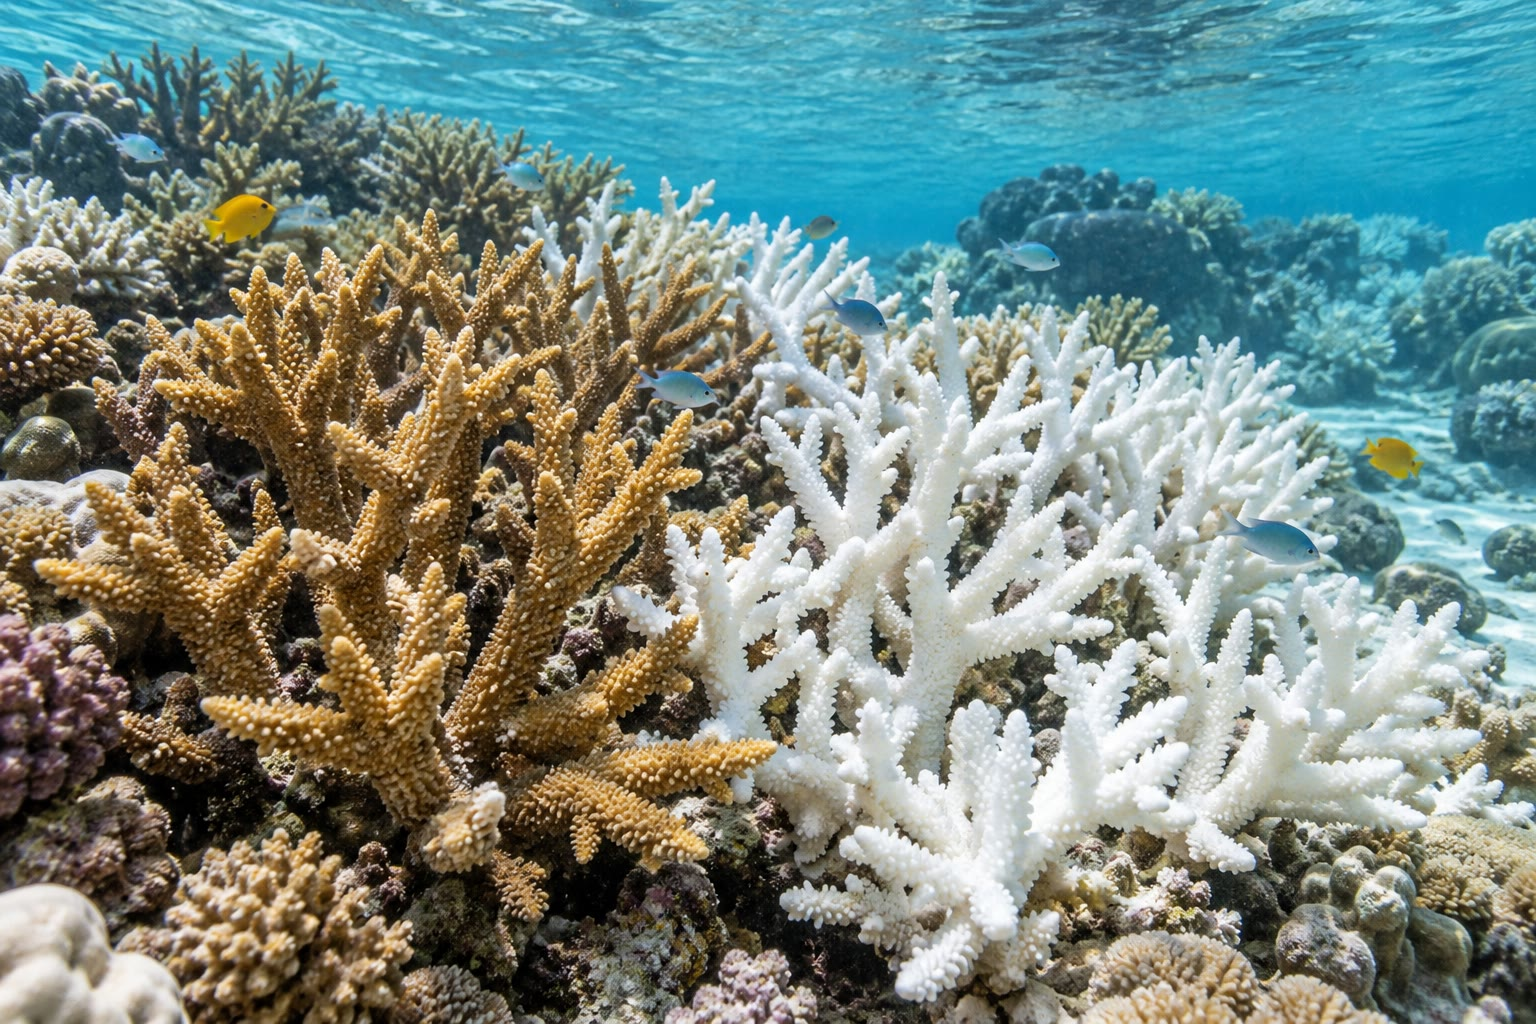
\includegraphics[width=0.44\linewidth]{images/book4/ai/b4-27-coral-bleaching.jpg}\hspace{0.04\linewidth}
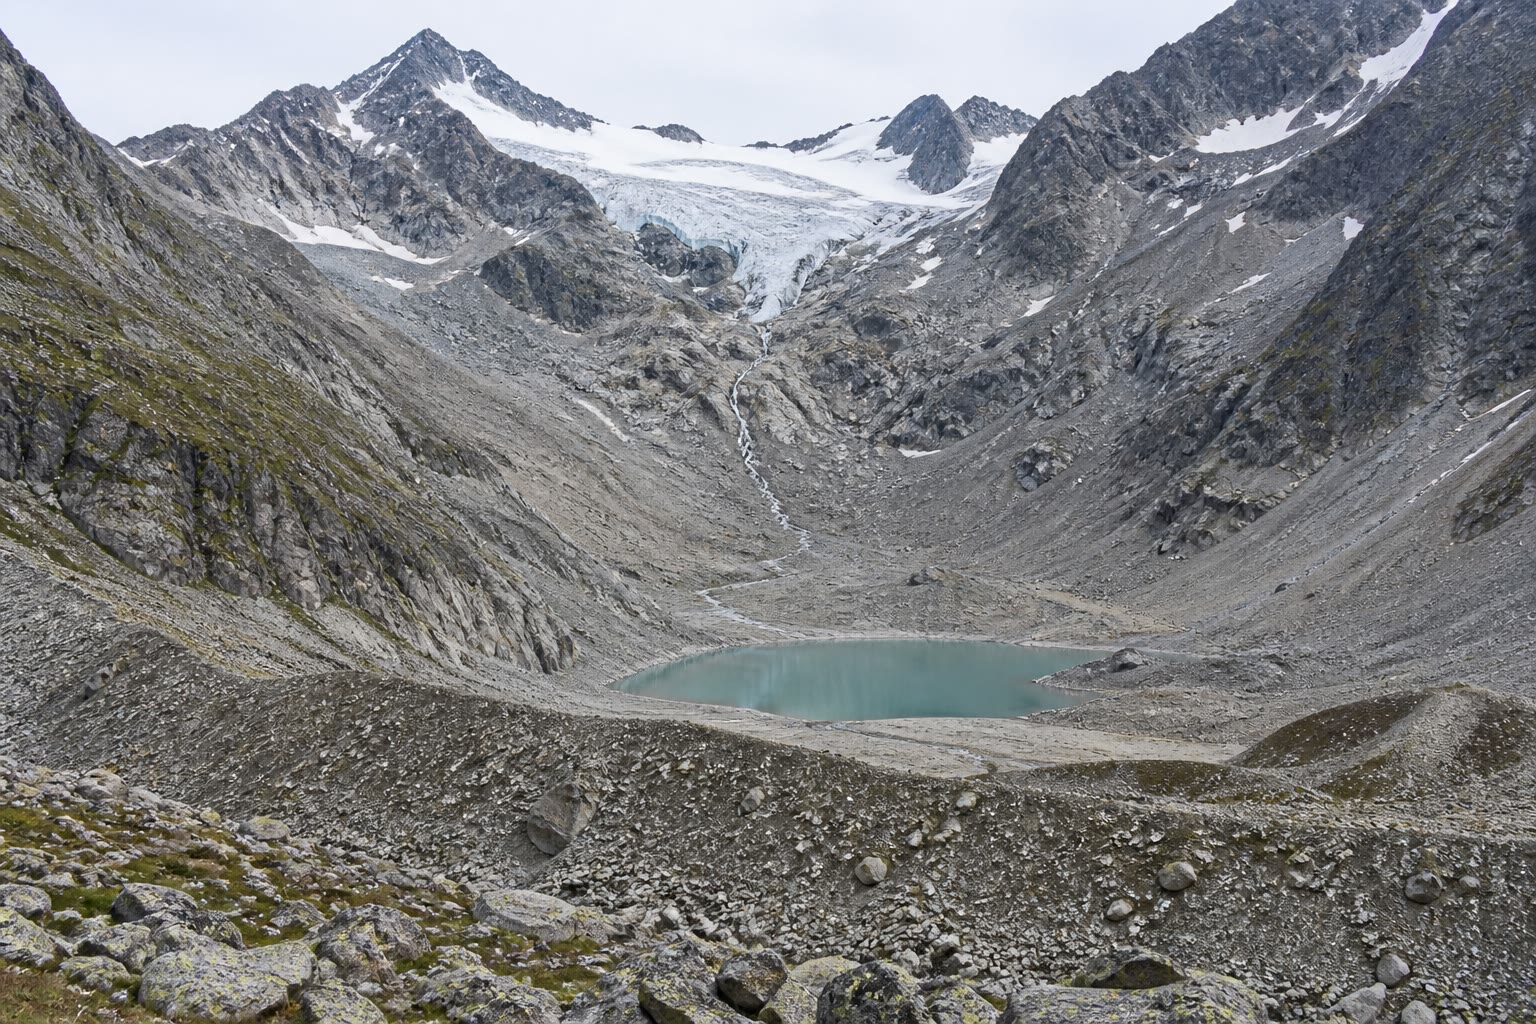
\includegraphics[width=0.44\linewidth]{images/book4/ai/b4-27-glacier-retreat.jpg}

{\small 两支“温度计”。左：白化的珊瑚礁，珊瑚的白色
骨骼透过已失去藻类的组织显露出来。右：一条
山谷冰川已沿谷地向上退缩，留下裸露的岩石，
岩石裸露处一个世纪前曾为冰体所覆盖。}
\end{omfigure}

\section{账本：灭绝及其估算}

\begin{theorem}[物种–面积关系与栖息地丧失的代价]\label{thm:b2:global-change:sar}
\index{物种–面积关系}\index{灭绝速率}\index{栖息地丧失}\index{灭绝债务}
发现于面积为 $A$ 的区域中的物种数，随面积的幂增长，
即 $S = cA^{z}$，对岛屿与栖息地片段，$z \approx 0.25$（面积
加倍使物种增加约五分之一；面积增大百倍，
物种增至三倍）。若栖息地缩减至原范围的 $1 - h$ 比例，
则它最终能容纳的物种数
降至原数的 $(1 - h)^{z}$：
损失一半栖息地将使其物种减少 \qty{16}{\%}，
损失 \qty{90}{\%} 则减少 \qty{44}{\%}，损失 \qty{99}{\%} 则减少
\qty{68}{\%}。损失并非立即显现——片段中的幸存者仍能存活一段时间，
即\emph{\omterm{thm:b2:global-change:sar}{灭绝债务}}，在数十年间逐步偿清，小种群
因\omterm{thm:b2:population-genetics:drift}{遗传漂变}与\omterm{prop:b2:population-genetics:inbreeding}{近交}而相继消亡（见
\cref{ch:b2:population-genetics}）——这也是估算当前\omterm{thm:b2:global-change:sar}{灭绝速率}的基础：
当前\omterm{thm:b2:global-change:sar}{灭绝速率}为化石记录中背景速率的一百至一千倍，背景速率约为
每年每百万种中有一种，
而如今每年正在消失数千种，
在约一千万种之中。
\end{theorem}
\begin{proof}
$S'/S = (A'/A)^{z} = (1 - h)^{z}$；取 $z = 0.25$，$0.5^{0.25} =
0.84$，$0.1^{0.25} = 0.56$，$0.01^{0.25} = 0.32$。该关系式
本身是经验性的，其指数反映了岛屿上
新物种迁入（随岛屿趋于饱和而减少）与
原有物种灭绝（随其种群缩小而增加）之间
的平衡，即麦克阿瑟与威尔逊
理论中的平衡。
\end{proof}
\begin{proof}[证据]
喀拉喀托群岛诸岛经 1883 年火山喷发
几近毁尽生命，此后植物、鸟类与昆虫重新定居，
经演替，于五十年内达到
按面积预测的物种数；辛伯洛夫与
威尔逊于 1966 年在佛罗里达熏蒸过的红树林小岛，一年内
物种数恢复原状，但物种已不尽相同。巴西大西洋
森林面积缩减至 \qty{10}{\%}，已损失
或几近损失了该关系式所预测的鸟类物种比例；在
世界自然保护联盟评估过的每一类群中，四分之一至三分之一的物种受到威胁——鸟类
占 \qty{13}{\%}，哺乳动物 \qty{27}{\%}，两栖动物 \qty{41}{\%}，珊瑚
占 \qty{44}{\%}——\omterm{thm:b2:global-change:sar}{栖息地丧失}为首要原因，
狩猎、\omterm{prop:b2:global-change:invasion}{外来物种}与污染，
以及日益突出的气候变化则为其余原因。
\end{proof}

\begin{omfigure}
\begin{tikzpicture}
\begin{loglogaxis}[
  width=0.68\linewidth, height=5.4cm,
  axis x line=bottom, axis y line=left,
  xmin=1, xmax=100000, ymin=5, ymax=200,
  xlabel={岛屿面积（\unit{km^2}）}, ylabel={陆生鸟类物种数},
  xlabel style={font=\small, at={(axis description cs:0.5,-0.13)}, anchor=north},
  ylabel style={font=\small},
  tick label style={font=\small},
  clip=false,
]
\addplot[only marks, mark=*, mark size=2pt, omDef] coordinates {(1.5,9) (8,14) (35,22) (150,32) (400,37) (1200,52) (4000,70) (13000,92) (35000,125) (85000,160)};
\addplot[very thick, omThm, domain=1:100000, samples=2] {9*x^0.25};
\node[font=\scriptsize, omThm, anchor=north west, align=left] at (axis cs:2,120) {$S = 9A^{0.25}$：面积增加百倍，\\ 物种数增至三倍};
\end{loglogaxis}
\end{tikzpicture}

{\small \omterm{thm:b2:global-change:sar}{物种–面积关系}，此处以某群岛岛屿上的陆生鸟类为例：
在对数坐标轴上呈斜率 $z = 0.25$ 的直线。若将栖息地切割至
原来的十分之一，久而久之，它能保留的物种
仅略多于一半。}
\end{omfigure}

\begin{proposition}[入侵、服务与可行之策]\label{prop:b2:global-change:invasion}
\index{外来物种}\index{生态系统服务}\index{减缓}\index{净零排放}
船舶、飞机与贸易已将数千种物种
越过了使其相隔的屏障；多数无法定居，但
少数成功者——澳大利亚的兔子、五大湖中的斑马贻贝、
使关岛鸟类绝迹的棕树蛇、
使九十种两栖动物走向
灭绝的壶菌——它们以恒定速度推进的前沿方式扩散，$c =
2\sqrt{rD}$，适用于以速率 $r$ 增长、
以扩散系数 $D$ 扩散的种群（斯凯拉姆的麝鼠，于
1905 年在布拉格附近放出，以每年 \qty{11}{km} 的速度扩散遍及欧洲，
其分布半径随时间呈直线增长）。与此相对的是生物圈
为其唯一的麻烦物种所做的贡献：
为四分之三的作物\omterm{def:b2:angiosperm-reproduction:pollination}{传粉}、净化水体、调蓄洪水、
固定氮素、形成\omterm{def:b2:living-soil:soil}{土壤}、渔业，
森林与\omterm{def:b2:living-soil:soil}{土壤}所储存的碳——\emph{\omterm{prop:b2:global-change:invasion}{生态系统服务}}
若能标价，其价值超过世界的
经济产值。可以采取的措施，由上述数字即可推出。
变暖在净排放停止时才会停止，不会更早。
在\cref{ch:b2:biogeochemical-cycles}中的\omterm{thm:b2:biogeochemical-cycles:box}{箱式模型}
对\emph{\omterm{prop:b2:global-change:invasion}{净零排放}}只允许一种理解。陆地在一定限度内可有所帮助——
再造林与\omterm{def:b2:living-soil:soil}{土壤}每年可封存一吉吨碳，持续几十年，
而化石燃料每年排放十吉吨；物种亦可
得到帮助而迁移，或被保留于足够大且相互连通的保护区，
使\omterm{thm:b2:global-change:sar}{物种–面积关系}与小种群的漂变不致将其灭绝。
本书所用的工具正是这些：
保护区的\omterm{def:b2:population-genetics:frequencies}{种群遗传学}、入侵物种的竞争、
作物的\omterm{thm:b2:global-change:phenology}{物候学}，以及\omterm{def:b2:living-soil:soil}{土壤}的收支。
\end{proposition}

\begin{example}[三种未来]\label{ex:b2:global-change:scenarios}
若排放维持在每年 \qty{10}{GtC}，至 2100 年将再增加 \qty{800}{GtC}，
加上已排放的 \qty{700}{}：$1.65\times 1.5 =
\qty{2.5}{\celsius}$，至本世纪末仍在上升。
若排放于 2070 年前降至零，将再增加约 \qty{250}{GtC}：\qty{1.6}{\celsius}，
随后持平。若先将排放加倍，如本世纪初几十年间那样，
则升温达 \qty{4}{\celsius} 或更多。温带的分布范围
在第一种情形下向今日之外移动 \qty{200}{km}，
第二种情形下移动 \qty{60}{km}；春季提前二十五天，
或提前六天；表层 pH 达到 $7.8$，或维持在接近
$8.0$ 的水平；灭绝估计依栖息地与升温共同而定，
其范围为十分之一至三分之一的物种。
两种未来的差别，即一条曲线下的累积面积，
也就是尚未作出的各项决定之和。
\end{example}

\section{练习}

\begin{exercise}[$\star$]\label{exo:b2:global-change:1}
叙述升温与\omterm{prop:b2:global-change:tcre}{累积排放}之间的关系，并
计算\omterm{prop:b2:global-change:tcre}{累积排放}为 700、1000 和
\qty{2000}{GtC} 时的升温。
\end{exercise}

\begin{exercise}[$\star$]\label{exo:b2:global-change:2}
定义度日与\omterm{thm:b2:global-change:phenology}{物候错配}，并
以捕蝇鸟为例。
\end{exercise}

\begin{exercise}[$\star$]\label{exo:b2:global-change:3}
等温线每升温一度，沿山坡向上与向极地方向各移动多远，
以及山顶物种为何无法跟随迁移？
\end{exercise}

\begin{exercise}[$\star$]\label{exo:b2:global-change:4}
用三句话说明向海洋中加入 \ensuremath{\mathrm{CO_2}} 为何会降低其 pH 与碳酸盐含量，
以及哪些生物会受到伤害。
\end{exercise}

\begin{exercise}[$\star\star$]\label{exo:b2:global-change:5}
计算升温为 \qty{1.5}{\celsius} 与
\qty{2}{\celsius} 时剩余的\omterm{prop:b2:global-change:tcre}{碳预算}，取 $\lambda = \qty{1.65}{\celsius}$ 每
\qty{1000}{GtC}，已排放 \qty{700}{GtC}；将两者均换算为
以每年 \qty{10}{GtC/yr} 计的年数。
\end{exercise}

\begin{exercise}[$\star\star$]\label{exo:b2:global-change:6}
春季自基温起升温，每天 $b = \qty{0.12}{\celsius}$，基温为
\qty{5}{\celsius}；某蛾需要 $K = 150$ 度日。计算由跨越基温至羽化所需的
天数，以及升温
\qty{1.5}{\celsius} 时羽化的提前量。
\end{exercise}

\begin{exercise}[$\star\star$]\label{exo:b2:global-change:7}
某植物的分布范围为 \qtyrange{800}{1400}{m}，位于一座高
\qty{1800}{m} 的山上，山体面积每随海拔升高 \qty{300}{m} 减半。
升温 \qty{3}{\celsius} 后，该分布带位于何处，损失了多少面积？
升温 \qty{5}{\celsius} 后又如何？
\end{exercise}

\begin{exercise}[$\star\star$]\label{exo:b2:global-change:8}
计算表层 pH 与氢离子浓度的增幅，
分别在 \qty{560}{ppm}、\qty{800}{ppm} 与 \qty{1000}{ppm} 时，由 $\mathrm{pH} = 8.2 -
0.9\log_{10}(p/280)$ 计算。
\end{exercise}

\begin{exercise}[$\star\star$]\label{exo:b2:global-change:9}
取 $z = 0.25$，当栖息地的
\qty{70}{\%}、\qty{95}{\%} 与 \qty{99.9}{\%} 被毁坏时，最终损失的物种比例各为多少？
为何即时损失较小？
\end{exercise}

\begin{exercise}[$\star\star\star$]\label{exo:b2:global-change:10}
某入侵物种以每年 $r = 0.7$ 的速率增长，扩散系数为 $D =
\qty{20}{km^2/yr}$。计算其前沿速度，以及穿越宽 \qty{1000}{km} 的国家所需时间。
使速度减半的是将 $r$ 减半，
还是将 $D$ 减半？
\end{exercise}

\begin{exercise}[$\star\star\star$]\label{exo:b2:global-change:11}
背景灭绝率为每百万物种年 1 次，
共有 800 万个物种。计算背景水平下每年与每世纪的预期灭绝数，
以及背景水平 1000 倍时的相应数值。
与上个世纪记录在案的一万次灭绝相比较，
并评论其中的差异。
\end{exercise}

\begin{exercise}[$\star\star\star$]\label{exo:b2:global-change:12}
“净排放停止，升温即停止。”试依据大气的\omterm{thm:b2:biogeochemical-cycles:box}{箱式模型}，
以及升温与\omterm{prop:b2:global-change:tcre}{累积排放}成正比的关系加以论证，
并指出该论证缺少什么。
\end{exercise}

\section{问题：2100 年的生物圈}

\begin{problem}[{周末问题——两条排放路径延伸至 2100 年，
各自的升温、由此引起的春季变化、
等温线移动的距离、投入海洋的酸，
以及森林所损失的物种，最后给出两种升温、两个 pH 值，
以及损失物种的比例}]
\label{pb:b2:global-change:1}
数据。$\lambda = \qty{1.65}{\celsius}$ 每 \qty{1000}{GtC}；
截至 2020 年已排放 \qty{700}{GtC}（升温 \qty{1.2}{\celsius}）。路径
A：每年 \qty{10}{GtC/yr} 恒定至 2100 年。路径 B：线性下降，
至 2070 年降至零。春季以每天 $b = \qty{0.1}{\celsius}$ 升温，
基温为 \qty{5}{\celsius}；一棵树需要 $K = 200$
度日方能展叶，一种迁徙鸟类于固定日期抵达，
即 2020 年该树展叶后 20 天。气温直减率
\qty{6.5}{\celsius/km}；纬向梯度 \qty{0.65}{\celsius}
每 \qty{100}{km}。海洋：$\mathrm{pH} = 8.2 - 0.9\log_{10}(p/280)$；
2100 年的 \ensuremath{\mathrm{CO_2}}：路径 A 为 \qty{600}{ppm}，路径 B 为 \qty{420}{ppm}。
一个面积为 \qty{e5}{km^2}、拥有 400 种树木的森林区域，$z = 0.25$，
至 2100 年时路径 A 下因砍伐损失其面积的 \qty{60}{\%}，
路径 B 下损失 \qty{20}{\%}。

\medskip
\noindent\textbf{第一部分——变暖。}
\begin{enumerate}
  \item 计算每条路径下 2100 年的累计排放量。
  \item 计算每条路径下 2100 年的升温幅度。
  \item 计算两条路径下 2050 年的升温幅度。
  \item 路径 A 下每十年的升温速率是多少？与
        观测到的每十年 \qty{0.2}{\celsius} 相比如何？
  \item 在路径 B 下，升温是否会在 2070 年停止？
        依据比例关系说明原因。
  \item 与 \qty{2}{\celsius} 对应的累计排放量是多少，
        路径 A 在哪一年达到该值？
\end{enumerate}

\medskip
\noindent\textbf{第二部分——春季。}
\begin{enumerate}[resume]
  \item 计算 2020 年从基温跨越到展叶所需的天数。
  \item 计算两条路径下 2100 年展叶相对 2020 年的提前量
        （以相对 2020 年的升温计）。
  \item 鸟类的抵达日期不变，计算
        2100 年两条路径下展叶与抵达之间的间隔。
  \item 该鸟所需的毛毛虫在展叶后 15 天达到高峰，
        持续 10 天。
        在哪一条路径下鸟仍能找到它们？
  \item 假设鸟类改为每升温一度提前 \qty{3}{d}，
        重新计算路径 A 下的间隔。
  \item 用一句话说明：威胁这只鸟的是错配，
        而不是升温本身。
\end{enumerate}

\medskip
\noindent\textbf{第三部分——分布范围。}
\begin{enumerate}[resume]
  \item 计算两条路径下等温线相对 2020 年
        在海拔与纬度上的位移。
  \item 某树种每年扩散 \qty{100}{m}。
        在路径 A 下，它能否跟上向极地移动的等温线？在路径 B 下呢？
  \item 某物种占据 \qtyrange{1500}{1800}{m} 的分布带，
        该山高 \qty{2000}{m}。路径 A 下，其分布带
        在 2100 年位于何处？会发生什么？
  \item 山地面积每 \qty{300}{m} 便减半。计算
        该物种在路径 B 下所损失的面积因子。
  \item 一种海洋鱼类每十年可跟随等温线移动 \qty{30}{km}。
        在路径 A 下，这已足够吗？
  \item 解释为什么即使物种能够耐受高温，
        其分布范围的下缘仍会后退。
\end{enumerate}

\medskip
\noindent\textbf{第四部分——海洋与森林。}
\begin{enumerate}[resume]
  \item 计算两条路径下 2100 年的表层 pH，
        以及自 1750 年以来氢离子浓度的上升幅度。
  \item 热带表层海水的\omterm{thm:b2:global-change:acid}{饱和度} $\Omega$ 在 1750 年为
        4，并随 $[\ensuremath{\mathrm{H^{+}}}]^{-1}$ 下降。计算
        2100 年两条路径下的值，并说明其对珊瑚意味着什么。
  \item 计算该森林区域最终能够容纳的树种数，
        并给出两条路径下各自的损失数。
  \item 升温还会带来额外损失：假设相对 2020 年每升温一度，
        又使尚存物种减少 \qty{5}{\%}。重新计算
        两条路径下剩余的物种数。
  \item 给出两条路径下 400 种树木中损失的比例。
  \item 在每条路径下，砍伐与升温两种原因中
        哪一种占主导？
  \item 陈述结论：2100 年两条路径下的升温幅度、pH
        以及损失的树种比例。
\end{enumerate}
\end{problem}
